\chapterbegin{Prueba en entorno real}
\label{chp:entornoReal}
\minitoc
\sectionx{Introducci�n}

Esta prueba consiste en simular el funcionamiento de la red en un entorno lo m�s parecido a lo que se enfrentar�a. Para ello se ha instalado el concentrador en un punto fijo como se observa en la figura \ref{fig:pruebaLocalizacion} (marcador central del c�rculo) y el nodo se ha ido cambiando de posici�n. Con esta prueba se ha comprobado el alcance de la red, el env�o de los mensajes de la web f�sica por Bluetooth y las reconexiones de los nodos a la red.

\begin{figure}[h]
	\centering
	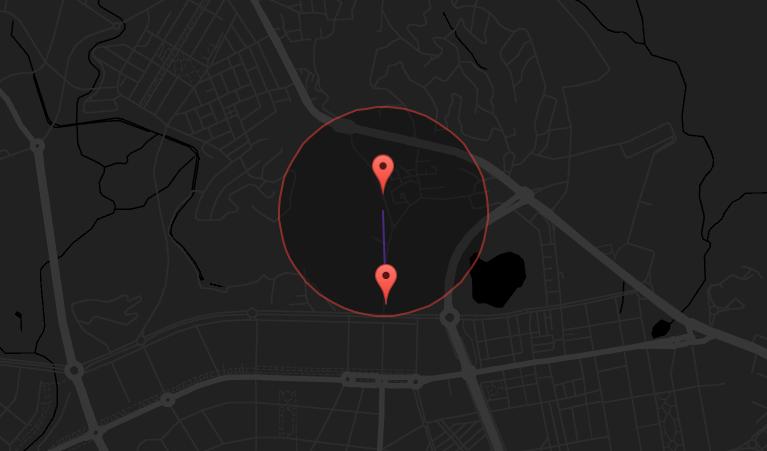
\includegraphics[width=0.7\textwidth]{graphs/pruebaLocalizacion}
	\caption{Posici�n del concentrador y nodo durante la prueba en el punto de m�ximo alcance}
	\label{fig:pruebaLocalizacion}
\end{figure}

\sectionx{Metodolog�a}

C�mo se ha indicado anteriormente, el concentrador se ha ubicado en un punto fijo que estuviera elevado, por ello se ha situado en el balc�n de la 2� planta de un edificio. Y el nodo se ha ido cambiado de posici�n hasta llegar a la distancia m�xima y que este perdiera la conexi�n con el concentrador, despu�s de esto se ha vuelto a acercar para comprobar la reconexi�n a la red.

\sectionx{Resultados}

Despu�s de realizar las pruebas se ha estimado la distancia m�xima a la que el nodo puede situarse para poder mantener la conexi�n que es de 400m, pero esta medida mejorar�a cambiando la antena y utilizando un amplificador en transmisi�n lo que quedar� como una l�nea futura de mejora de este proyecto.\\

En cuanto a la reconexi�n del nodo, ha sido todo un �xito. Despu�s de repetir la desconexi�n y reconexi�n del nodo var�as veces en todas de ellas la ha realizado sin problemas. Y adem�s no ha dejado de enviar los mensajes de la web f�sica en ning�n momento durante la prueba.\\
\begin{figure}[h]
	\centering
	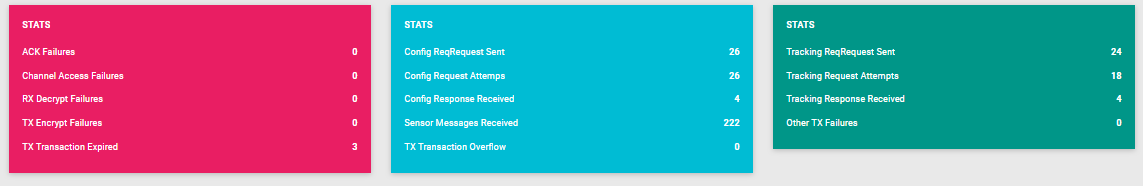
\includegraphics[width=0.8\textwidth]{graphs/pruebaEstadisticas}
	\caption{Estad�sticas de la red despu�s de la prueba}
	\label{fig:pruebaEstadisticas}
\end{figure}
Finalmente en la figura \ref{fig:pruebaEstadisticas} se observan las estad�sticas que ha recogido la red despu�s de las pruebas,  donde se tiene que el concentrador ha recibido 26 peticiones del nodo para que le env�e la configuraci�n (esta petici�n se realiza despu�s de una conexi�n o reconexi�n)  y 222 mensajes de tipo "Sensor" que son los que el nodo env�a peri�dicamente con datos de temperatura, bater�a, estad�sticas y algunos par�metros m�s.




\chapterend{}